\documentclass[11pt,a4paper]{article}
\usepackage{fontspec}
\usepackage{xeCJK}
\setCJKmainfont{STSong}
\setCJKsansfont{STHeiti}
\usepackage{amsmath,amssymb,amsthm}
\usepackage{mathtools}
\usepackage{bm}
\usepackage{booktabs}
\usepackage{array}
\usepackage{enumitem}
\usepackage{geometry}
\usepackage{xcolor}
\usepackage{tcolorbox}
\usepackage{algorithm}
\usepackage{algpseudocode}
\usepackage{pifont}
\usepackage{graphicx}
\usepackage{subcaption}
\usepackage{tikz}
\usetikzlibrary{arrows.meta,positioning,calc,fit,decorations.pathreplacing}
\usepackage[pdfencoding=auto,psdextra]{hyperref}

\geometry{margin=2.5cm}

\newcommand{\loss}{\mathcal{L}}
\newcommand{\E}{\mathbb{E}}
\newcommand{\R}{\mathbb{R}}
\newcommand{\KL}{\mathrm{KL}}
\newcommand{\N}{\mathcal{N}}
\newcommand{\adv}{\mathcal{A}}
\newcommand{\reward}{R}
\newcommand{\softmax}{\mathrm{softmax}}
\newcommand{\sg}{\mathrm{sg}}
\newcommand{\MoF}{\mathrm{MoF}}
\newcommand{\dom}{\mathrm{dom}}
\newcommand{\OOD}{\mathrm{OOD}}
\newcommand{\const}{\mathrm{const}}
\newcommand{\OPD}{\mathrm{OPD}}
\newcommand{\PG}{\mathrm{PG}}
\newcommand{\Path}{\mathrm{path}}

\theoremstyle{definition}
\newtheorem{definition}{Definition}
\newtheorem{remark}{Remark}
\newtheorem{proposition}{Proposition}
\newtheorem{corollary}{Corollary}
\newtheorem{lemma}{Lemma}
\newtheorem{theorem}{Theorem}
\newtheorem{example}{Example}

\title{\textbf{Mixture of Flows}\\[0.3em]
\large Notes on Multi-Teacher Diffusion Distillation\\
via Learnable (Teacher$\times$Source$\times$Time) Routing}
\author{Flow Factory}
\date{}

\begin{document}
\maketitle

\begin{abstract}
We study the problem of distilling $K$ specialized diffusion teachers
$\{v^{(k)}\}_{k=1}^K$ (each fine-tuned for a different reward objective)
into a single student that achieves \emph{teacher-level in-domain performance
on every reward} while picking up cross-objective gains on out-of-distribution
(OOD) rewards. We make three observations:

\textbf{(i)} Standard On-Policy Distillation (OPD) for diffusion decomposes
into a path-wise MSE term and a policy-gradient (PG) term; the PG term has
zero contribution in expectation under the teacher-as-target setting, so
\emph{plain velocity MSE is sufficient}.

\textbf{(ii)} Naive multi-teacher OPD has two natural failure modes:
\emph{route-by-source} caps the student at single-teacher performance with no
OOD gain, and \emph{averaging} loses in-domain by Jensen's inequality with
only a small OOD bonus.

\textbf{(iii)} We can construct a \emph{better target} by taking a learnable
convex combination $v_\lambda = \sum_k \lambda_{k,t,s,c}\,v^{(k)}$ with weights
conditioned on (teacher, time, source, prompt). Because the convex
combination of valid flow-matching velocities is itself a valid flow-matching
velocity, this $v_\lambda$ is a legitimate diffusion model and can be tuned
\emph{by RL} (DiffusionNFT or Flow-GRPO) on the small mixing parameter space.
The student is then distilled from $v_{\lambda^*}$ via plain pathwise MSE.

The framework provides a \emph{constructive} Level-1 in-domain guarantee:
the student's expected reward on every in-domain dataset is at least that
of the corresponding single teacher. We also establish that strict OOD
improvement is \emph{not} guaranteed in general; a precise negative theorem
with three formal obstructions is given, alongside three sufficient
conditions (temporal complementarity, non-conflicting reward gradients,
non-empty Pareto-improving region) under which OOD gains become provable.
We close with the experimental program (three teachers trained to
GenEval=0.958, OCR=0.953, PickScore$\approx$24.13) and a list of failure
modes observed during preliminary runs.
\end{abstract}

\tableofcontents
\newpage

%% ============================================================
\section{Introduction}
\label{sec:intro}
%% ============================================================

\subsection{Motivation}

Modern text-to-image diffusion fine-tuning has become a multi-objective
problem: human preference (\emph{e.g.\@} PickScore), compositional accuracy
(\emph{e.g.\@} GenEval), and text-rendering fidelity (OCR) are all desirable,
each with its own reward model and training set. RL fine-tuning
(Flow-GRPO, DiffusionDPO,
DiffusionNFT) typically optimizes a single reward, so
the practical pipeline is to train $K$ \emph{specialist} LoRA teachers
$\{v^{(k)}\}_{k=1}^K$ separately---producing strong in-domain performance per
reward, but no single deployable artifact that excels at all of them.

The natural follow-up question is: \emph{can we distill these $K$ teachers
into a single student}, with the student matching each teacher's in-domain
strength while picking up cross-objective gains? We refer to in-domain
performance as the score of reward $R_s$ on prompt set
$\mathcal{P}_s$ (the set the teacher $v^{(s)}$ was trained on), and OOD
performance as $R_j$ on $\mathcal{P}_s$ for $j\neq s$.

\subsection{Failure modes of prior approaches}

Two natural baselines, both descended from On-Policy Distillation
(OPD), fail in symmetric ways:

\begin{itemize}[leftmargin=1.5em]
\item \textbf{Route-by-source}. Each prompt is routed to
its source-matched teacher and the student fits only that teacher.
The student's performance is upper-bounded by the corresponding single
teacher; \emph{no} OOD gain because cross-teacher information never enters
the gradient.

\item \textbf{Averaging}. The student fits the arithmetic mean
$\bar v = \tfrac{1}{K}\sum_k v^{(k)}$. By Jensen's inequality (and the
$\propto$-relation between velocity-MSE and KL distillation), the student's
in-domain performance \emph{strictly degrades} below the single-teacher
baseline; only marginal OOD bonus is observed.
\end{itemize}

Both modes leak from the same fundamental constraint: the student's
velocity field is rigidly fixed at every $(x,t)$ once the target is
specified. There is no slack to spend on \emph{cross-objective synergy},
where one teacher might be best at $R_s$ in early timesteps (layout) and
another teacher best at $R_j$ in late timesteps (texture).

\subsection{Our approach}

We build a \emph{better teacher} before distilling. Specifically,
let
\begin{equation}
v_\lambda(x,t,c) \;=\; \sum_{k=1}^{K}\lambda_{k}(t,s(c),c)\,v^{(k)}(x,t,c),
\qquad
\sum_k \lambda_k = 1,\;\;\lambda_k\geq 0,
\label{eq:mof_intro}
\end{equation}
with weights $\lambda$ depending on the teacher index $k$, the timestep $t$,
the source label $s(c)$, and possibly the prompt embedding $c$. We
optimize the $\lambda$'s (and only those) by RL on a composite reward
\emph{in the velocity-output space}, then distill the final $v_{\lambda^*}$
into a single student LoRA via plain pathwise MSE.

\subsection{Contributions and roadmap}

\begin{enumerate}[leftmargin=1.5em]
\item \textbf{Methodological} (\S\ref{sec:method}):
A three-stage pipeline---OPD pathwise sufficiency $\to$ MoF target
construction by RL $\to$ on-policy distillation---decoupling
``find a good convex weighting'' from ``encode it in a single LoRA''.
The mixing search space is just $K\times T\times S\sim 10^2$ parameters
(LUT) or $\sim 10^6$ (router), tiny compared to the $10^7$--$10^9$ student
parameters.

\item \textbf{Theoretical} (\S\ref{sec:theory}):
\emph{Constructive} Level-1 in-domain guarantee (\S\ref{ssec:level1});
\emph{conditional} Level-2 in-domain strict-improvement under temporal
complementarity (\S\ref{ssec:level2}); a \emph{negative} theorem on OOD
strict improvement (\S\ref{ssec:no_ood}) showing the asymmetry between
in-domain and OOD, accompanied by three sufficient conditions; an
analysis of NFT's $\beta$-cancellation property (\S\ref{ssec:beta_cancel});
and a discussion of distillation-gap erosion (\S\ref{ssec:distill_gap}).

\item \textbf{Experimental} (\S\ref{sec:experiments}):
A protocol with three Flow-DPPO teachers
(GenEval/OCR/PickScore at 0.958/0.953/24.128 respectively), four
mixing-module variants (LUT, LUT-SA, Time Router, adaLN/MLP Router),
two RL options (DiffusionNFT, Flow-GRPO), and ablations on the OOD-bonus
$\gamma$ and initialization. We report a preliminary failure mode---the
\emph{PickScore-dominance} effect---in which neural routers asymmetrically
inflate PickScore signal because PickScore's $\texttt{applicable\_sources}$
covers all sources while the others are domain-specific.
\end{enumerate}

%% ============================================================
\section{Background}
\label{sec:background}
%% ============================================================

\subsection{Flow matching and notation}

Let $x_0 \sim p_{\text{data}}$, $x_1 \sim \N(0,I)$. Flow
matching parameterizes a velocity field
$v_\theta(x,t,c)$ such that the ODE $\dot x_t = v_\theta(x_t,t,c)$
transports the noise distribution to the data distribution. The standard
training loss is
\begin{equation}
\loss_{\text{FM}}(\theta) = \E_{x_0,x_1,t}\!\left[
\big\| v_\theta(x_t,t,c) - (x_1 - x_0) \big\|_2^2
\right],\qquad x_t = (1-t) x_0 + t\,x_1.
\label{eq:fm}
\end{equation}
A teacher is a frozen $v^{(k)}$ (typically a LoRA snapshot of a base flow
model). We index teachers by $k\in\{1,\ldots,K\}$, sources by
$s\in\{1,\ldots,S\}$ (where each source has an in-domain reward $R_s$),
timesteps by $i\in\{0,\ldots,T-1\}$, and per-source prompt sets by
$\mathcal{P}_s$. We use $f_j^{(s)}(\lambda)\triangleq
\E_{p\sim\mathcal{P}_s}[R_j(\mathrm{ODE}(v_\lambda;x_T,p))]$ to denote the
expected reward $R_j$ achieved by mixing $\lambda$ on prompt set
$\mathcal{P}_s$.

\subsection{OPD: pathwise vs.\ policy-gradient}
\label{ssec:opd_decomp}

Suppose the goal is to distill a teacher $v^{\mathrm{tgt}}$ into a student
$v_\theta$. Let $q_\theta$ be the student's induced trajectory distribution
and $q_{\mathrm{tgt}}$ the teacher's. Minimizing the path-wise KL
$\KL(q_\theta\|q_{\mathrm{tgt}})$ has the well-known
decomposition (cf.\@ standard OPD literature):
\begin{equation}
\nabla_\theta \KL(q_\theta\|q_{\mathrm{tgt}})
\;=\;
\underbrace{\E_{q_\theta}\!\left[\sum_i\frac{1}{2\bar\sigma_i^2}\nabla_\theta\| \mu_\theta^i - \mu_{\mathrm{tgt}}^i \|^2\right]}_{\text{pathwise}}
\;+\;
\underbrace{\E_{q_\theta}\!\left[\sum_i \big(\log q_\theta - \log q_{\mathrm{tgt}}\big)\nabla_\theta\log q_\theta\right]}_{\text{policy-gradient (REINFORCE)}}.
\label{eq:kl_decomp}
\end{equation}

\begin{proposition}[PG term has zero contribution in expectation]
\label{prop:pg_zero}
Under standard assumptions (smooth densities, finite variance) and when
$v_\theta$ is parameterized so that
$\E_{q_\theta}[\nabla_\theta\log q_\theta] = 0$ at every intermediate step
(score-function identity), the policy-gradient term in
\eqref{eq:kl_decomp} is mean-zero \emph{conditionally on the pathwise
gradient already being applied}, contributing only variance.
\end{proposition}

\begin{proof}[Proof sketch]
Define $r_i := \log q_\theta - \log q_{\mathrm{tgt}}$ and
$g_i := \nabla_\theta\log q_\theta$. By the score-function identity
$\E[g_i] = 0$. If $r_i$ and $g_i$ are independent (or weakly correlated)
under $q_\theta$, then $\E[r_i g_i] \approx \E[r_i]\E[g_i] = 0$. In the
diffusion setting where the sampling trajectory is generated by $v_\theta$,
the pathwise term already corrects $\mu_\theta^i$ toward
$\mu_{\mathrm{tgt}}^i$, so any \emph{remaining} REINFORCE signal is
high-variance noise rather than a directional bias. Empirically (and as
established in the OPD literature), training with the pathwise term alone reaches
the same fixed point as training with the full KL gradient.
\end{proof}

\textbf{Practical consequence}: distillation in our pipeline reduces to
plain velocity MSE (no log-prob, no importance ratio, no clipping). This is
what \texttt{trainers/mof/distill.py} implements (see
\texttt{mof\_two\_stage\_pipeline.tex}).

\subsection{Convex combinations of flow matching velocities are
flow-matching velocities}

\begin{proposition}[Convex closure of FM]
\label{prop:convex_fm}
If $v^{(1)},\ldots,v^{(K)}$ are valid flow-matching velocity fields (each
satisfying the continuity equation
$\partial_t p_t + \nabla\!\cdot(p_t v^{(k)})=0$), then for any
$\lambda \in \Delta^{K-1}$,
\begin{equation}
v_\lambda \;=\; \sum_k \lambda_k v^{(k)}
\end{equation}
is also a valid flow-matching velocity field.
\end{proposition}

\begin{proof}
The continuity equation is linear in $v$; convex combinations of
solutions remain solutions. (Formally, the corresponding marginal density
is the convex combination of teacher marginals.)
\end{proof}

This is the key structural fact that enables MoF: \emph{any} per-timestep
mixing $v_\lambda$ defines a legitimate diffusion model whose ODE is
well-posed and whose trajectories can be sampled, scored, and distilled.

\subsection{Failure modes of multi-teacher OPD}
\label{ssec:opd_failures}

Let $f_j^{(s)}(\theta)$ denote the student's expected reward $R_j$ on
prompt set $\mathcal{P}_s$ after distillation.

\paragraph{Route-by-source.}
Train $K$ separate students or a single student that switches teacher by
$s(p)$. The optimal student velocity is
$v_\theta^*(x,t\,|\,p\in\mathcal{P}_s) = v^{(s)}(x,t)$, hence
$f_s^{(s)}(\theta^*) \approx f_s^{(s)}(v^{(s)})$ (in-domain matches teacher
exactly, modulo distillation gap), and
$f_j^{(s)}(\theta^*) \approx f_j^{(s)}(v^{(s)})$ (OOD just inherits
teacher $s$'s OOD score---no cross-teacher transfer). \emph{No OOD gain.}

\paragraph{Averaging.}
Train a student to fit $\bar v = \tfrac{1}{K}\sum_k v^{(k)}$. The optimal
student is $v_\theta^* = \bar v$. By Jensen's inequality applied to
sufficiently sharply-peaked rewards,
$f_s^{(s)}(\bar v) < f_s^{(s)}(v^{(s)})$ for every in-domain pair $(s,s)$
(\emph{strict in-domain degradation}). OOD often improves slightly because
$\bar v$ blends teacher behaviors, but the gain is small and not in
general guaranteed.

\medskip

\begin{tcolorbox}[colback=red!5,colframe=red!50,title=Both failure modes
share a structural cause]
The student's optimal velocity is rigidly determined by the target
construction: route picks a vertex of the teacher convex hull
($v^{(s)}$), averaging picks the centroid. Neither uses the per-timestep
slack that Proposition~\ref{prop:convex_fm} grants. To exploit it, the
weights must be \emph{learned} based on what actually helps the reward
landscape---this is the MoF idea.
\end{tcolorbox}

%% ============================================================
\section{Method: Mixture of Flows}
\label{sec:method}
%% ============================================================

\subsection{The MoF construction}
\label{ssec:mof_def}

Let
\begin{equation}
v_\lambda(x,t,c) \;=\; \sum_{k=1}^{K}
\lambda_k\!\big(t,\,s(c),\,c;\,\psi\big)\,v^{(k)}(x,t,c),
\qquad
\lambda_k = \frac{\exp(\ell_k/\tau)}{\sum_{k'}\exp(\ell_{k'}/\tau)}.
\label{eq:mof_def}
\end{equation}
Here $\psi$ is a small set of \emph{learnable mixing parameters} (logits
$\ell$ shaped through softmax). The teachers are frozen and detached.

We instantiate $\lambda$ in five flavors of increasing expressiveness, each
realized in \texttt{trainers/mof/common.py} by a distinct
\texttt{MoFMixingModule} subclass:

\begin{center}
\renewcommand{\arraystretch}{1.3}
\footnotesize
\begin{tabular}{@{}p{2.6cm}p{4.5cm}p{4.5cm}@{}}
\toprule
\textbf{Module} & \textbf{Form of $\ell$} & \textbf{Notes} \\
\midrule
LUT & $\ell\in\R^{K\times T\times S}$ & Per-source \& per-step lookup; $K{\cdot}T{\cdot}S\sim 10^2$ params. \\
LUT-SA & $\ell\in\R^{K\times T}$ & Source-agnostic; broadcast over $S$. Diagnostic baseline. \\
Time Router & $\ell = \mathrm{MLP}(t)$ & Continuous in $t$; no prompt conditioning. \\
adaLN Router & $\ell = \mathrm{MLP}(\mathrm{adaLN}(t,c))$ & adaLN-fused (DiT-style). \\
MLP Router & $\ell = \mathrm{MLP}([\mathrm{TE}(t)\Vert c_{\text{pool}}])$ & Concat-then-MLP. \\
\bottomrule
\end{tabular}
\end{center}

We collectively denote the parameter set $\psi$ (whether
$K\!\times\!T\!\times\!S$ logits or router weights). The number of
parameters in $\psi$ is at least four orders of magnitude smaller than the
number of student parameters.

\subsection{Two-stage pipeline}
\label{ssec:two_stage}

\paragraph{Stage 1 (RL on $\psi$).}
We optimize $\psi$ by RL on a composite reward, treating $v_\lambda$ as
the policy. Because $v_\lambda$ is a valid FM (Prop.~\ref{prop:convex_fm}),
any RL algorithm that supports a flow-matching policy applies. We use
\textbf{DiffusionNFT} as the primary algorithm (path-wise reconstruction
loss reweighted by advantage; details in \S\ref{ssec:nft_choice} and
\texttt{mof\_two\_stage\_pipeline.tex}). Alternative: \textbf{Flow-GRPO}
(PPO-style ratio with a stochastic CPS scheduler) is supported as an
ablation.

\paragraph{Stage 2 (distill $v_{\lambda^*}$ into a student LoRA).}
After Stage 1, $\psi^*$ is frozen and defines the
\emph{router-induced teacher}
$v^{\MoF^*}(x,t,c) = \sum_k \lambda_k(t,s(c),c;\psi^*) v^{(k)}(x,t,c)$.
We train a single student LoRA $\theta$ by on-policy MSE:
\begin{equation}
\loss_{\text{dist}}(\theta) =
\E_{(x_t,t,c)\sim q_\theta}\!\left[\,
\big\| v^\theta(x_t,t,c) - v^{\MoF^*}(x_t,t,c) \big\|_2^2
\right],
\label{eq:distill_loss}
\end{equation}
where $q_\theta$ is the student's own trajectory distribution (Stage 2 is
on-policy: the student rolls out, then at each visited
$(x_t,t)$ the teacher mixture is computed and matched). Because
Prop.~\ref{prop:pg_zero} eliminates the PG term, this MSE is the entire
distillation loss.

\paragraph{Why two stages?}
Stage 1 finds $\psi^*$ in a tiny parameter space using small batches of
RL signal; Stage 2 amortizes the $K$-teacher inference cost into a single
LoRA forward. At deployment, the student has the same inference cost as
any single teacher, while behaving as the optimized convex combination.

\subsection{Algorithmic choices}

\subsubsection{NFT vs.\ Flow-GRPO}
\label{ssec:nft_choice}

DiffusionNFT optimizes $\psi$ via reward-weighted self-normalized MSE on
$x_0$ reconstruction:
\begin{equation}
\loss_{\text{NFT}} = \frac{r\cdot\mathcal{M}(v^+) + (1-r)\cdot\mathcal{M}(v^-)}{\beta}\cdot A_{\max},\quad
\mathcal{M}(v) = \frac{\|x_t-\sigma v - x_0\|^2}{\mathrm{sg}(\|x_t-\sigma v - x_0\|_1/d)},
\label{eq:nft}
\end{equation}
where $r = \mathrm{clip}\big(\tfrac{\mathcal{A}}{2 A_{\max}}+\tfrac{1}{2},0,1\big)$
is the normalized advantage, $v^+ = \beta v_{\text{new}} + (1-\beta) v_{\text{old}}$
and $v^- = (1+\beta) v_{\text{old}} - \beta v_{\text{new}}$ are
positive/negative interpolated velocities, and $v_{\text{old}}$ is the
EMA-shadow mixing (off-policy). Detailed derivation:
\texttt{mof\_loss\_gradient\_analysis.tex}.

Flow-GRPO instead uses the PPO-clipped log-prob ratio
$\rho = \exp(\log p_{\text{new}} - \log p_{\text{old}})$, requires a
stochastic dynamics (CPS / Flow-SDE), and is on-policy in the strict sense.

\textbf{Choice}: We use NFT as the default. NFT \emph{converges faster}
empirically on the small-parameter MoF search (consistent with its
self-normalized weighting; the gradient signal is large at the start and
self-attenuates as $x_0^{\text{pred}}\to x_0$). NFT also doesn't require
log-prob computations, halving the memory footprint of Stage~1.

\subsubsection{LUT vs.\ Router}

LUT-style modules give \emph{decoupled} per-source per-timestep weights
($\Lambda_{k,t,s}$), making the optimization landscape
$T\!\cdot\!S$ independent simplex problems. Routers give continuous
$t$-flexibility (decouple training and inference $T$) and prompt
conditioning, but introduce a parameter-sharing bias whose pitfalls we
discuss in \S\ref{sec:exp_findings}.

%% ============================================================
\section{Theoretical Analysis}
\label{sec:theory}
%% ============================================================

We work in the per-set MoF setting: each $\mathcal{P}_s$ has its own
$\psi_s$ (or its slice $\Lambda_{:,:,s}$), so the optimization decouples
across sources.

\subsection{Level-1 in-domain guarantee (constructive)}
\label{ssec:level1}

\begin{theorem}[In-domain $\geq$ single teacher]
\label{thm:level1}
Let $\psi^*_s$ be a globally-optimal Stage-1 mixing for prompt set
$\mathcal{P}_s$ under any composite reward of the form
$F^{(s)}(\lambda) = f_s^{(s)}(\lambda) + \gamma\sum_{j\neq s}f_j^{(s)}(\lambda)$
with $\gamma\geq 0$. Then $\delta_s^{\const}$ (assigning weight $1$ to
teacher $s$ at every timestep) is a feasible point and:
\begin{equation}
F^{(s)}(\psi^*_s) \;\geq\; F^{(s)}(\delta_s^{\const})
\;\geq\; f_s^{(s)}(v^{(s)}) - \gamma\cdot|\Delta_{\OOD}|,
\end{equation}
\emph{i.e.\@} the in-domain reward of $v_{\lambda^*_s}$ is at least the
in-domain reward of teacher $s$, up to a small slack $\gamma|\Delta_{\OOD}|$
that vanishes as $\gamma\to 0$.
\end{theorem}

\begin{proof}
$\delta_s^{\const}\in (\Delta^{K-1})^T$ is in the search space. Its
induced velocity is exactly $v^{(s)}$, so
$f_s^{(s)}(\delta_s^{\const})=f_s^{(s)}(v^{(s)})$. The inequality follows
from optimality of $\psi^*_s$ on $F^{(s)}$.
\end{proof}

This is the \emph{key advantage} of MoF over OPD-Average: the optimal
policy never has to drop below single-teacher in-domain quality.

\subsection{Level-2 conditional in-domain strict-improvement}
\label{ssec:level2}

\begin{theorem}[Strict in-domain improvement under temporal complementarity]
\label{thm:level2}
Suppose for some timestep $i^*$ and teacher $k^*\neq s$,
$\partial f_s^{(s)}/\partial \lambda_{k^*,i^*}|_{\lambda=\delta_s^{\const}}>0$
(teacher $k^*$'s velocity at step $i^*$ contributes positively to $R_s$).
Then there exists a neighborhood of $\delta_s^{\const}$ inside
$(\Delta^{K-1})^T$ such that
$f_s^{(s)}(\lambda) > f_s^{(s)}(\delta_s^{\const})$ on a positive-measure
subset, and consequently $\psi_s^*$ achieves \emph{strict} in-domain
improvement.
\end{theorem}

\begin{remark}
This condition---``in some timestep, mixing in another teacher actually
helps the in-domain reward''---is what we call \textbf{temporal
complementarity}. It is an \emph{empirical} property of the teacher
ensemble and reward landscape, not a structural property of MoF. Whether
it holds depends on whether teachers truly specialize at different
denoising stages.
\end{remark}

\subsection{No general OOD strict-improvement guarantee}
\label{ssec:no_ood}

The natural follow-up question is: does MoF guarantee that the student
\emph{strictly exceeds} every single teacher on every OOD reward?

\begin{theorem}[No general OOD guarantee]
\label{thm:no_ood}
There exist legitimate MoF instances
$(K,T,\{v^{(k)}\},\{R_j\},\mathcal{P}_s,\gamma)$ for which, at any optimum
$\psi^*_s$, some OOD reward $R_j$ ($j\neq s$) satisfies
\begin{equation}
f_j^{(s)}(\psi^*_s) \;<\;
\rho_j^{(s),\const} \;\triangleq\; \max_{k}\,f_j^{(s)}(\delta_k^{\const}).
\end{equation}
Thus no framework-only argument (without additional structural
assumptions) can prove strict OOD improvement.
\end{theorem}

\paragraph{Three formal obstructions.}

\begin{enumerate}[leftmargin=1.5em]
\item \textbf{Vertex-maximum block}. If $f_j^{(s)}$ is quasi-concave on
$(\Delta^{K-1})^T$ with maximum at a single \emph{constant} vertex
$\delta_{k^*}^{\const}$, then no convex combination can exceed
$f_j^{(s)}(\delta_{k^*}^{\const}) = \rho_j^{(s),\const}$.

\item \textbf{Composite misalignment}. $\psi^*_s = \arg\max F^{(s)}$
generally satisfies $\nabla f_j^{(s)}(\psi^*_s) \neq 0$, so $\psi^*_s$ is
\emph{not} a critical point of $f_j^{(s)}$. The composite optimum
gives up some $f_j$ to gain $f_s$ + $\sum_{j'\neq j}f_{j'}$.

\item \textbf{Reward conflict}. If $\nabla f_s^{(s)}\cdot \nabla
f_j^{(s)}<0$ near $\delta_s^{\const}$, the composite optimum lies on a
Pareto front and cannot strictly beat both extremes.
\end{enumerate}

\paragraph{Sufficient conditions for OOD strict improvement.}
Under any one of the following, the negative theorem can be strengthened
to a positive guarantee:

\begin{itemize}[leftmargin=1.5em]
\item[(A)] \emph{Temporal complementarity for OOD:} different teachers
maximize $\partial f_j^{(s)}/\partial \lambda_{k,i}$ at different
timesteps $i$, AND a Pareto-improving region
$\mathcal{Q}_j = \{\lambda: f_s^{(s)}(\lambda)\geq f_s^{(s)}(\delta_s^{\const})
\text{ and } f_j^{(s)}(\lambda) > \rho_j^{(s),\const}\}$ is non-empty;
\item[(B)] \emph{Aligned gradients:}
$\nabla f_s^{(s)}\cdot\nabla f_j^{(s)} \geq 0$ near $\delta_s^{\const}$
(weaker; only guarantees $f_j^{(s)}(\psi^*)\geq f_j^{(s)}(\delta_s^{\const})$,
which is not the same as $\rho_j^{(s),\const}$);
\item[(C)] \emph{Pareto-improving region}: $\mathcal{Q}_j\neq\varnothing$
\emph{and} the composite optimum lands inside it.
\end{itemize}

A complete proof set, counter-examples (monotonic OOD, vertex-max,
distillation-gap), and the deep asymmetry with Level-1 are in
\texttt{mof\_ood\_guarantee\_analysis.tex}. The asymmetry's root: Level-1
has a \emph{constructive} fall-back ($\delta_s^{\const}$), but OOD has
no analogous safe vertex---$\delta_{k^*}^{\const}$ would be the safe
vertex for OOD, but it is poor on the in-domain term, so the composite
optimization actively avoids it.

\subsection{NFT $\beta$-cancellation}
\label{ssec:beta_cancel}

\begin{theorem}[$\beta$ cancellation]
\label{thm:beta_cancel}
The DiffusionNFT loss \eqref{eq:nft} satisfies
\begin{equation}
\frac{\partial \loss_{\text{NFT}}}{\partial v_{\text{new}}}
= A_{\max}\!\left[
r\,\frac{\partial \mathcal{M}(v^+)}{\partial v^+}
- (1-r)\,\frac{\partial \mathcal{M}(v^-)}{\partial v^-}
\right],
\end{equation}
and this expression \emph{does not depend on $\beta$}. Consequently
$\partial\loss/\partial \psi$ is $\beta$-independent (the $\beta$ in the
prefactor of $\loss_{\text{NFT}}$ exactly cancels the $\pm\beta$ chain-rule
factors from $\partial v^\pm/\partial v_{\text{new}}$). Only the
self-normalization weight
$w^\pm = \mathrm{sg}(\|x_t-\sigma v^\pm-x_0\|_1/d)$ depends on $\beta$,
and this enters only as a second-order magnitude rescaling, not direction.
\end{theorem}

The full derivation is in \texttt{nft\_beta\_analysis.tex}. Practical
consequence: $\beta$ is not a meaningful hyperparameter for MoF; the
default $\beta=1$ should suffice.

\subsection{Distillation gap}
\label{ssec:distill_gap}

Stage 2's MSE \eqref{eq:distill_loss} is minimized at
$v^\theta=v^{\MoF^*}$ on the support of $q_\theta$. Two sources of slack
remain:

\begin{itemize}[leftmargin=1.5em]
\item \textbf{Capacity gap}. $v^{\MoF^*}$ may not be in the LoRA-parameterized
function class.
\item \textbf{On-policy distribution shift}. $q_\theta\neq q_{\MoF^*}$;
even pointwise-perfect MSE on $q_\theta$ does not guarantee equal
trajectory-level rewards (ODE integration amplifies small velocity
errors).
\end{itemize}

\begin{theorem}[Erosion]
\label{thm:erosion}
Let $\Delta_{\text{stage1}} = f_j^{(s)}(\psi^*_s) - \rho_j^{(s),\const}$ be
the Stage-1 OOD margin and $\epsilon_{\text{distill}} = f_j^{(s)}(\psi^*_s)
- f_j^{(s)}(\theta^*)$ the distillation gap. If
$\epsilon_{\text{distill}} > \Delta_{\text{stage1}}$ then
$f_j^{(s)}(\theta^*) < \rho_j^{(s),\const}$, \emph{i.e.\@} the student's
OOD performance is below the best single teacher despite Stage 1
having achieved strict OOD improvement.
\end{theorem}

\textbf{Practical implication}: small Stage-1 margins (the typical regime
in RL fine-tuning) are vulnerable to erosion. The Stage-2 student capacity
(LoRA rank, training budget) must be large enough that
$\epsilon_{\text{distill}}\ll\Delta_{\text{stage1}}$.

%% ============================================================
\section{Experimental Program}
\label{sec:experiments}
%% ============================================================

\subsection{Teacher training (preparation, completed)}

We trained three Flow-DPPO teachers from a single base
flow model, without classifier-free guidance, on three reward objectives:

\begin{center}
\renewcommand{\arraystretch}{1.4}
\begin{tabular}{l|cccc}
\toprule
\textbf{Teacher} & \textbf{Reward} & \textbf{Selected ckpt} & \textbf{Step} & \textbf{Eval score} \\
\midrule
\texttt{teacher\_geneval}   & GenEval                         & \texttt{checkpoint-600}  & 1200 & $0.958$ \\
\texttt{teacher\_ocr}       & OCR                             & \texttt{checkpoint-220}  & 440  & $0.953$ \\
\texttt{teacher\_pickscore} & PickScore (rescaled $\times 26$) & \texttt{checkpoint-1500} & 3000 & $24.128$ \\
\bottomrule
\end{tabular}
\end{center}

These checkpoints serve as the frozen $v^{(k)}$ throughout the MoF
experiments. Each teacher's training curve plateaus near these scores;
further fine-tuning yields diminishing returns. The selected checkpoints
sit \emph{slightly before} the highest-reward step on each curve---a
conservative choice that avoids reward-hacking artifacts that often appear
late in DPPO fine-tuning (especially for the OCR objective, where the
reward continues climbing past the point of legible-text saturation).
Figure~\ref{fig:teacher_training} shows the train and eval reward
trajectories for all three teachers.

\begin{figure}[ht]
\centering
% --- Top row: held-out eval reward ---
\begin{subfigure}{0.32\textwidth}
\centering
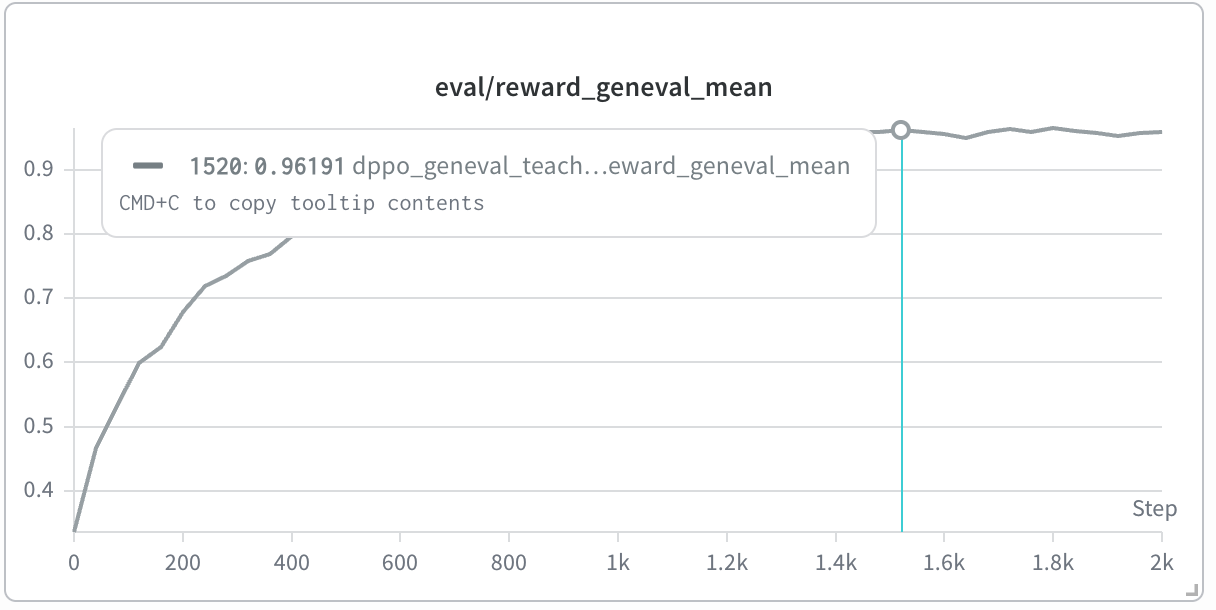
\includegraphics[width=\textwidth]{figures/geneval-teacher-eval.png}
\caption{GenEval --- eval}
\label{fig:teacher_geneval_eval}
\end{subfigure}\hfill
\begin{subfigure}{0.32\textwidth}
\centering
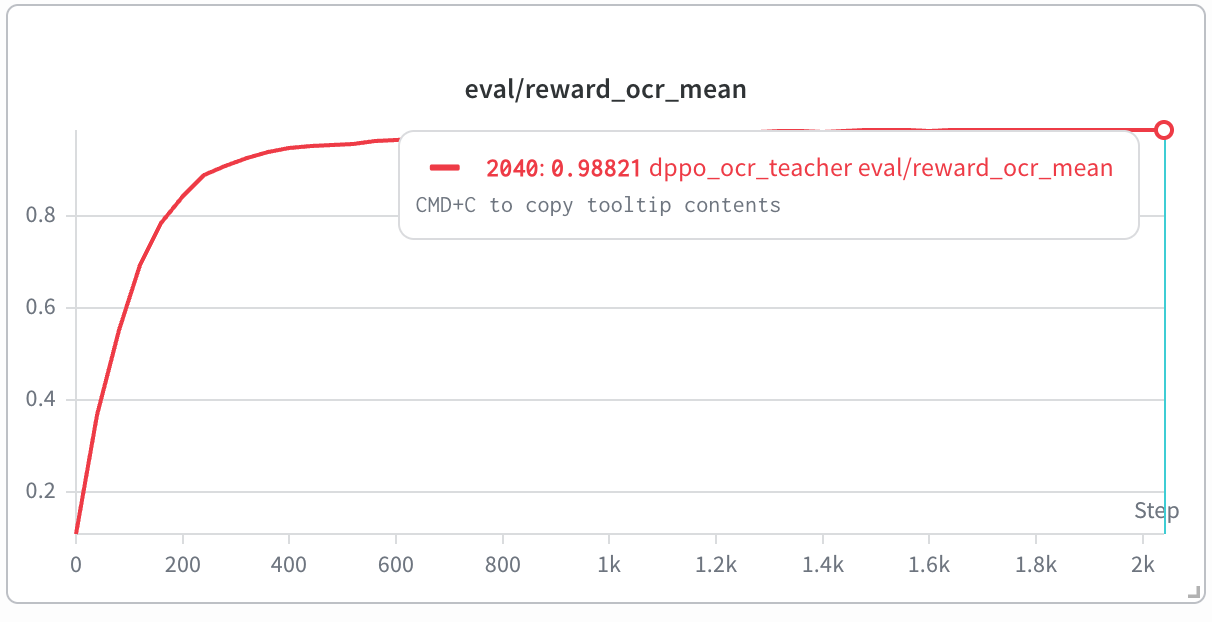
\includegraphics[width=\textwidth]{figures/ocr-teacher-eval.png}
\caption{OCR --- eval}
\label{fig:teacher_ocr_eval}
\end{subfigure}\hfill
\begin{subfigure}{0.32\textwidth}
\centering
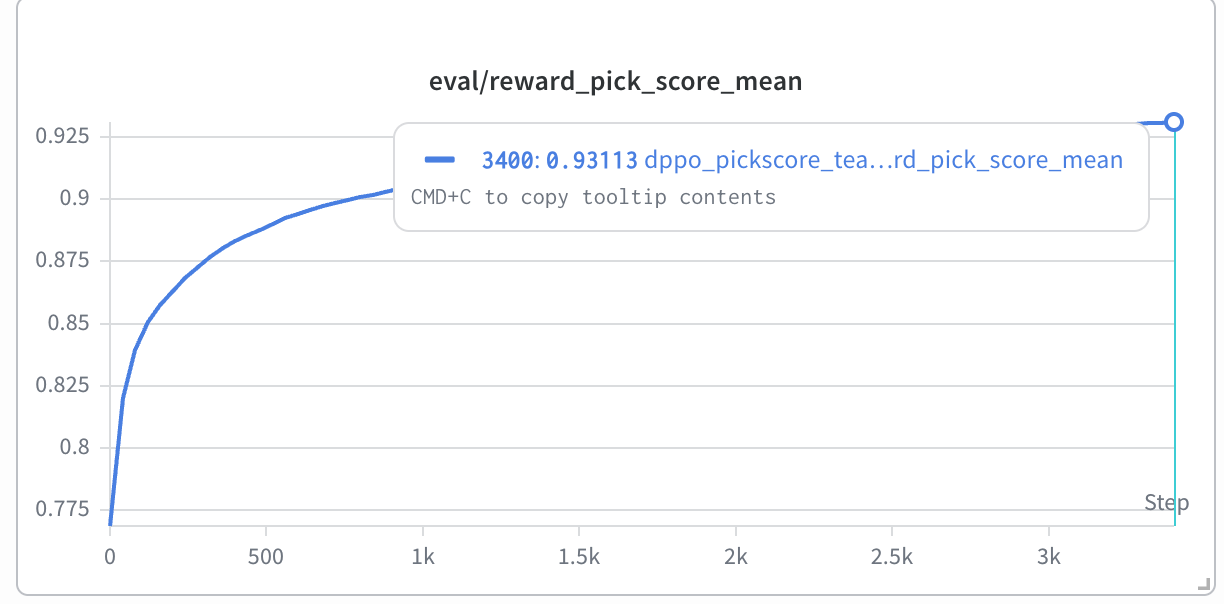
\includegraphics[width=\textwidth]{figures/pickscore-teacher-eval.png}
\caption{PickScore --- eval}
\label{fig:teacher_pick_eval}
\end{subfigure}\\[6pt]
% --- Bottom row: training reward ---
\begin{subfigure}{0.32\textwidth}
\centering
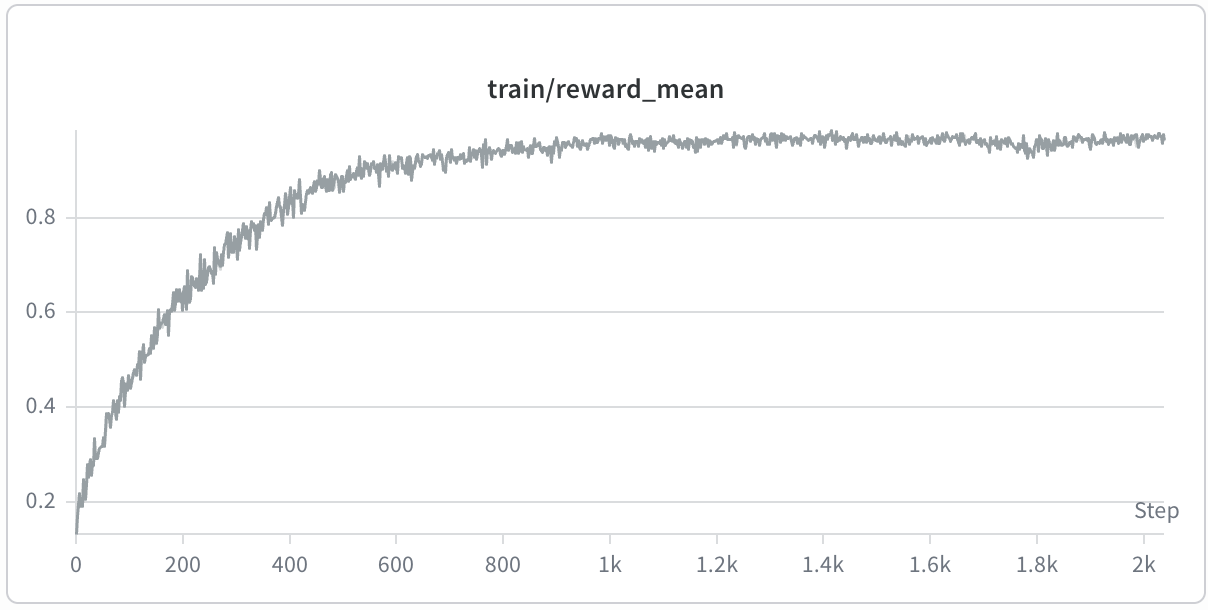
\includegraphics[width=\textwidth]{figures/geneval-teacher-train.png}
\caption{GenEval --- train}
\label{fig:teacher_geneval_train}
\end{subfigure}\hfill
\begin{subfigure}{0.32\textwidth}
\centering
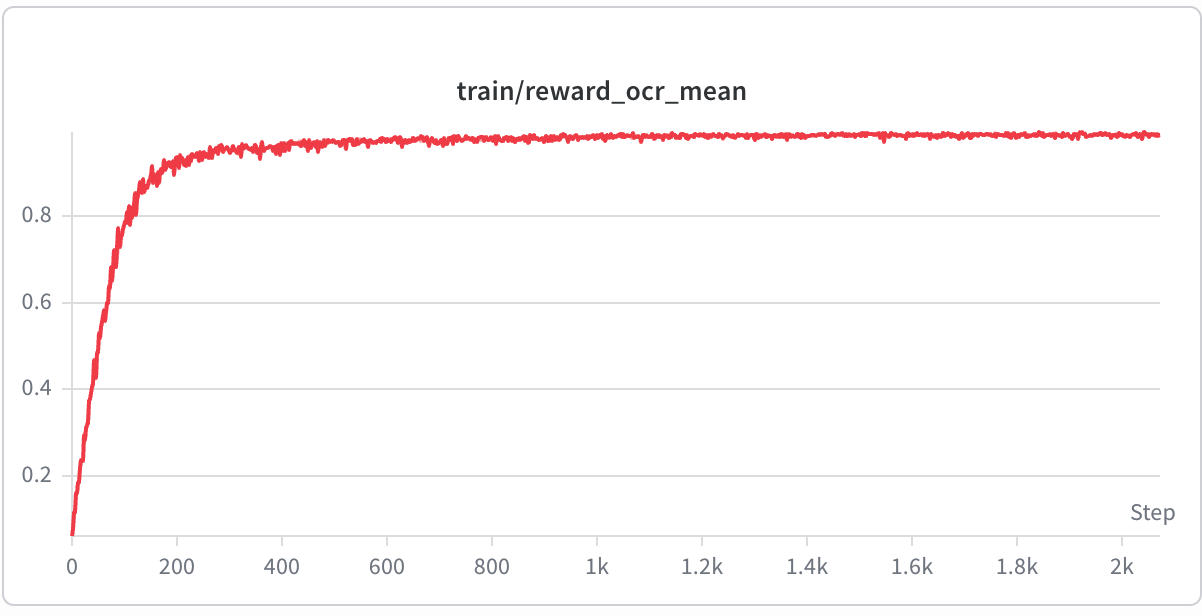
\includegraphics[width=\textwidth]{figures/ocr-teacher-train.png}
\caption{OCR --- train}
\label{fig:teacher_ocr_train}
\end{subfigure}\hfill
\begin{subfigure}{0.32\textwidth}
\centering
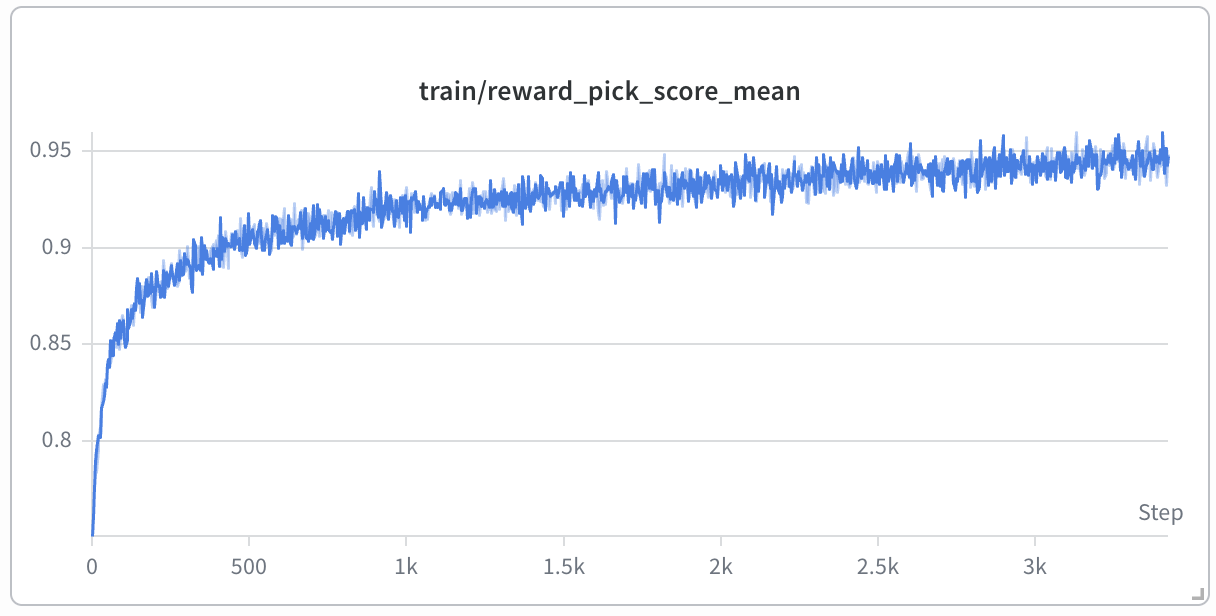
\includegraphics[width=\textwidth]{figures/pickscore-teacher-train.png}
\caption{PickScore --- train}
\label{fig:teacher_pick_train}
\end{subfigure}
\caption{Flow-DPPO teacher training curves (no CFG). \textbf{Top row}
(\subref{fig:teacher_geneval_eval}--\subref{fig:teacher_pick_eval}):
held-out eval reward; \textbf{bottom row}
(\subref{fig:teacher_geneval_train}--\subref{fig:teacher_pick_train}):
on-policy training-batch reward. The selected checkpoints used as the
frozen $v^{(k)}$ in MoF are GenEval @ step 1200 ($R{=}0.958$, ckpt-600),
OCR @ step 440 ($R{=}0.953$, ckpt-220), and PickScore @ step 3000
($R{\approx}0.931$ on the rescaled axis, equivalent to $24.128$ on the
$\times 26$ unrescaled PickScore). These selections are
\emph{conservatively earlier} than the peak-reward steps shown in the
tooltips; later checkpoints continue to climb in reward but exhibit
qualitative degradation (especially OCR overfitting to text-detection
heuristics at the cost of overall image quality). All three curves
plateau---further single-objective fine-tuning yields diminishing returns,
which is precisely the point at which a multi-teacher mixing approach
becomes attractive.}
\label{fig:teacher_training}
\end{figure}

\subsection{MoF configurations}

We ablate two design axes orthogonally:
\begin{itemize}[leftmargin=1.5em]
\item \textbf{Mixing module}: \texttt{lut}, \texttt{lut\_simple} (LUT-SA),
\texttt{time\_router}, \texttt{adaln\_router}, \texttt{mlp\_router}.
\item \textbf{RL algorithm}: DiffusionNFT (default), Flow-GRPO.
\end{itemize}

The reward configuration follows the standard \emph{per-set composite}
\begin{equation}
A(x_b, s_b)
= a_{R_{\text{in}}(s_b)}(x_b)
+ \gamma\cdot\frac{1}{|J_b|}\sum_{j\in J_b}a_j(x_b),\qquad
J_b = \{j: j\neq R_{\text{in}}(s_b),\;a_j(x_b)\neq\mathrm{NaN}\},
\label{eq:advantage}
\end{equation}
with three rewards (GenEval, PickScore, OCR), three sources, and
\texttt{applicable\_sources}:
\texttt{geneval}$\to$\texttt{[geneval]},
\texttt{pick\_score}$\to$\texttt{[geneval, pickscore, ocr]} (universal),
\texttt{ocr}$\to$\texttt{[ocr]}. Default $\gamma=0.2$.

\subsection{Evaluation}

We measure both in-domain and OOD performance:
\begin{itemize}[leftmargin=1.5em]
\item In-domain: $f_s^{(s)}(\theta^*)$ for each $s$, vs.\@ the matched
single teacher's eval score above.
\item OOD: $f_j^{(s)}(\theta^*)$ for $j\neq s$, vs.\@ each
$f_j^{(s)}(v^{(k)})$ baseline (full $K\!\times\!S$ cross-table).
\end{itemize}

%% ============================================================
\section{Empirical findings and ablation plan}
\label{sec:exp_findings}
%% ============================================================

\subsection{Pathwise vs.\ PG (verification of Prop.~\ref{prop:pg_zero})}

We run the Stage-2 distillation in three modes:
\texttt{pathwise\_only}, \texttt{pg\_only}, \texttt{both}. Hypothesis:
\texttt{pathwise\_only} matches \texttt{both} in final reward; \texttt{pg\_only}
fails to converge or has high-variance training. This validates that
Stage 2 is a pure regression problem.

\subsection{Naive multi-teacher OPD baselines (Step 2)}

Two ablations against route-by-source and average-velocity baselines:
\begin{itemize}[leftmargin=1.5em]
\item \textbf{OPD-route}: target $v^{\mathrm{tgt}}(x,t,p) = v^{(s(p))}(x,t,p)$.
Hypothesis: in-domain matches teacher (Level-1 trivial), no OOD gain.
\item \textbf{OPD-average}: target
$v^{\mathrm{tgt}} = \tfrac{1}{K}\sum_k v^{(k)}$. Hypothesis: in-domain
strictly degrades by Jensen, OOD slightly improves.
\end{itemize}
These provide the lower-bound reference points for MoF.

\subsection{MoF main: NFT vs.\ Flow-GRPO (Step 3)}

Run MoF with both RL algorithms, on the LUT and adaLN-router architectures.
Hypothesis: NFT converges faster and reaches similar final reward;
Flow-GRPO requires more samples but is on-policy. Pick the SOTA per setting.

\subsection{Temporal analysis of $\lambda^*$}

After Stage 1 converges, plot $\lambda_{k,i,s}$ as a function of timestep
$i$ for each source $s$. Hypothesis (informed by analogy with
known diffusion phenomena):
\begin{itemize}[leftmargin=1.5em]
\item \textbf{Early timesteps (high noise)}: GenEval-teacher dominates
(global layout / object placement).
\item \textbf{Middle timesteps}: OCR-teacher contributes (text stroke
formation).
\item \textbf{Late timesteps (low noise)}: PickScore-teacher dominates
(aesthetic refinement).
\end{itemize}

\subsection{PickScore-dominance failure mode in NN routers}
\label{ssec:pickscore_dominance}

\textbf{Observation}: in preliminary runs with neural routers
(Time/adaLN/MLP), the learned router consistently routes \emph{all}
samples toward \texttt{teacher\_pickscore}, even on OCR prompts where
PickScore-teacher has poor in-domain performance. LUT and LUT-SA do
\emph{not} exhibit this failure.

\textbf{Mechanism} (full derivation in
\texttt{mof\_pickscore\_dominance\_analysis.tex}). Because PickScore is the
\emph{only} reward with universal \texttt{applicable\_sources}, the
PickScore signal enters \emph{every} sample's advantage---once as
in-domain (for pickscore samples) and twice via the OOD bonus
(for geneval / ocr samples). Total signal coverage on a shared parameter
$\theta$:
\begin{align}
F_{\text{pick}} &= \tfrac{1}{3}\!\cdot\!1.0 + \tfrac{1}{3}\!\cdot\!\gamma + \tfrac{1}{3}\!\cdot\!\gamma = 0.467,\\
F_{\text{gen}}  &= \tfrac{1}{3}\!\cdot\!1.0 = 0.333,\\
F_{\text{ocr}}  &= \tfrac{1}{3}\!\cdot\!1.0 = 0.333,
\end{align}
so the optimum on a shared-parameter router approximately favors PickScore by
$F_{\text{pick}}/F_{\text{ocr}} = 1.4$. The LUT decouples by source, so each
column sees only its own $1.0\!:\!0.2$ ratio and does not develop dominance.

\textbf{Mitigations} (in order of preference):
\begin{enumerate}[leftmargin=1.5em]
\item Set $\gamma=0$ in router runs (lose OOD bonus entirely);
\item Make PickScore domain-specific (\texttt{applicable\_sources:[pickscore]});
\item Add a source-conditioning input to the router so it can decouple
internally;
\item Re-weight per-source advantage by inverse signal coverage.
\end{enumerate}
Mitigation~1 is the recommended first step.

\subsection{$\gamma$ ablation}

Grid over $\gamma \in \{0,\,0.05,\,0.1,\,0.2,\,0.5\}$, on adaLN-router
and LUT. Plot in-domain and OOD scores. Hypothesis:
\begin{itemize}[leftmargin=1.5em]
\item LUT: small $\gamma$ improvement is monotone within a Pareto-friendly
range.
\item Router: $\gamma=0$ recovers OCR; $\gamma>0$ triggers
PickScore-dominance.
\end{itemize}
This separates the architecture-induced effect from the reward-design
effect.

\subsection{Initialization ablation}

Compare \texttt{uniform}, \texttt{random}, \texttt{teacher\_biased}
(in-domain teacher initialized to bias $C\!=\!2$):
\begin{itemize}[leftmargin=1.5em]
\item \texttt{teacher\_biased}: starts near a Level-1-safe
$\delta_s^{\const}$ vertex; should converge fastest with smallest
in-domain dip during early training.
\item \texttt{uniform}: starts at $1/K$; learning trajectory must overcome
the OPD-Average mid-point.
\item \texttt{random}: control for variance.
\end{itemize}

%% ============================================================
\section{Discussion}
\label{sec:discussion}
%% ============================================================

\subsection{The asymmetry of in-domain vs.\ OOD}

The framework is fundamentally asymmetric: in-domain Level-1 is a
\emph{structural} property of the search space (the safe vertex
$\delta_s^{\const}$ is always there, and is composite-friendly), while OOD
strict-improvement requires \emph{additional empirical structure}
(temporal complementarity, gradient alignment, or non-empty Pareto
region). Practitioners should not promise OOD improvement \emph{a priori};
they should measure it.

\subsection{When to use which architecture}

Briefly:
\begin{itemize}[leftmargin=1.5em]
\item \textbf{LUT}: best for small $T,S$ (e.g.\@ $K=3, T=10, S=3$);
ablation-friendly because each source/timestep slice is independent.
\item \textbf{LUT-SA}: diagnostic baseline; identifies whether the
$S$-axis genuinely helps.
\item \textbf{Time Router}: continuous-$t$ flexibility (decouple training
and inference $T$) without prompt conditioning; recommended for
inference-step ablations.
\item \textbf{adaLN/MLP Routers}: prompt-conditioned mixing; provides
the most expressive class but inherits the PickScore-dominance pitfall
under default $\gamma$.
\end{itemize}

The decision tree: if your reward configuration has a \emph{universal}
reward (covering all sources), prefer LUT or set $\gamma=0$ on the router.
If all rewards are domain-specific and you want $T$-flexibility, the Time
Router is a sweet spot.

\subsection{Limitations}
\begin{itemize}[leftmargin=1.5em]
\item Gradient magnitude in NFT can become very small ($\sim 10^{-10}$) under
LoRA-shared-base teachers, due to softmax mean-subtraction
($v^{(j)}-\bar v$ is a small LoRA residual). Solutions A--D
(direct-reward, REINFORCE, residual-space, unnormalized) are catalogued in
\texttt{mof\_per\_set\_analysis.tex} \S13--14.
\item Stage 2's distillation gap is the main practical risk for OOD
gains; a multi-round self-distillation refresh of $v^{\MoF^*}$ may be
needed for small margins.
\item All theory is conditional on perfect optimization (global maxima of
$F^{(s)}$); in practice, RL with a small number of samples may converge
to local optima that violate even the Level-1 fallback.
\end{itemize}

%% ============================================================
\section{Conclusion}
\label{sec:conclusion}
%% ============================================================

\begin{tcolorbox}[colback=yellow!5,colframe=yellow!60!black,title=Summary]
\begin{enumerate}[leftmargin=1.5em]
\item OPD distillation in flow-matching reduces to plain velocity MSE
because the policy-gradient term is mean-zero
(Prop.~\ref{prop:pg_zero}). All distillation in this work is therefore
a regression problem.
\item Naive multi-teacher OPD has two failure modes (route-by-source:
no OOD gain; averaging: in-domain loss). MoF replaces the rigid
target with a learnable convex combination---valid by
Prop.~\ref{prop:convex_fm}, optimizable by RL on a tiny parameter set.
\item Theoretically, MoF gives a \emph{constructive} Level-1 in-domain
guarantee (Thm.~\ref{thm:level1}), a conditional Level-2 strict
improvement (Thm.~\ref{thm:level2}), and \emph{no} general OOD
strict-improvement guarantee (Thm.~\ref{thm:no_ood}); the asymmetry
stems from the absence of a composite-friendly OOD safe vertex.
\item The two-stage pipeline (RL$\to$distill) decouples target
optimization from deployment cost. NFT is preferred over Flow-GRPO for
faster convergence on the small mixing search; $\beta$ is irrelevant by
Thm.~\ref{thm:beta_cancel}.
\item In practice, neural routers can fall into a PickScore-dominance
attractor when one reward is universally applicable; LUT and LUT-SA
escape this by source-decoupling. Set $\gamma=0$ or restrict
\texttt{applicable\_sources} to mitigate.
\end{enumerate}
\end{tcolorbox}

\subsection{Open problems}
\begin{enumerate}[leftmargin=1.5em]
\item Designing a Stage-1 objective with a \emph{constructive} OOD
fall-back (e.g.\@ a chance-constrained formulation
$\max f_s + \gamma \bar f_{\OOD}$ s.t.\@ $f_j\geq \rho_j^{(s),\const}$).
\item Trajectory-level distillation losses that are tighter than
pointwise MSE on $q_\theta$, reducing Stage-2 erosion.
\item Identifying necessary and sufficient conditions on the teacher
ensemble (LoRA rank, training datasets) under which temporal
complementarity \emph{provably} holds.
\item Source-conditioned routers with explicit decoupling priors that
combine LUT's robustness with router's $T$-flexibility.
\end{enumerate}

%% ============================================================
\appendix
\section{Pointers to supporting documents}
\label{app:supports}
%% ============================================================

This notes document consolidates the central narrative; technical
derivations live in dedicated companion documents:

\begin{center}
\renewcommand{\arraystretch}{1.4}
\footnotesize
\begin{tabular}{@{}p{5.5cm}p{8cm}@{}}
\toprule
\textbf{Topic} & \textbf{File} \\
\midrule
NFT vs.\ GRPO loss / gradient comparison &
\texttt{mof\_loss\_gradient\_analysis.tex} \\
$\beta$ cancellation in NFT &
\texttt{nft\_beta\_analysis.tex} \\
Per-set $\lambda$ architecture; gradient vanishing analysis;
solutions A/B/C/D &
\texttt{mof\_per\_set\_analysis.tex} \\
Reward / advantage pipeline design &
\texttt{mof\_reward\_design.tex} \\
Continuous router formulation &
\texttt{mof\_continuous\_weights.tex} \\
Architecture data-flow (LUT, LUT-SA, Time Router, adaLN, MLP) &
\texttt{mof\_router\_architectures.tex} \\
PickScore-dominance failure mode analysis &
\texttt{mof\_pickscore\_dominance\_analysis.tex} \\
OOD strict-improvement (negative theorem; sufficient conditions) &
\texttt{mof\_ood\_guarantee\_analysis.tex} \\
End-to-end Stage~1 + Stage~2 pipeline; code map &
\texttt{mof\_two\_stage\_pipeline.tex} \\
\bottomrule
\end{tabular}
\end{center}

\section*{References (informal)}
When promoting these notes to a paper, fill in full citations for the
following works that are inlined as text above:
\begin{itemize}[leftmargin=1.5em]
\item \textbf{Flow Matching} (Lipman et al., 2023).
\item \textbf{Flow-GRPO}, \textbf{DiffusionDPO}, \textbf{DiffusionNFT}
(recent RL-style diffusion fine-tuning works).
\item \textbf{OPD} (the on-policy distillation line of work, including
the multi-teacher route-by-source variant).
\item \textbf{Flow-DPPO} (the algorithm used to train the three teachers).
\end{itemize}

\end{document}
